\section{Fist Experiment}
For this use case, we are going to use the dataset proposed by \textit{Giselsson et al.} in \cite{giselsson2017public}, which we are going to refer to as the ‘plant\_seedlings\_v2’ dataset. This dataset contains \textasciitilde 1000 RGB images with a resolution of 10 pixels per mm divided in 12 different plant species. The plants in the dataset are listed in table \ref{tab:dataset_species}. This dataset contains pictures of one of the most common weeds found in sugar beet plantations, a plant commonly referred to as ''charlock''. \cite{cioni_weed_2010}\\
Even though the dataset is mainly focused on seedlings and it contains pictures of other plants as well, this will give us proper insights of the models’ behaviours in a farming setting.
\begin{table}[ht]
\centering
\begin{tabular}{|c|c|c|}
\hline
    English & Latin \\
\hline
    Maize & Zea mays L.\\
    Common wheat & Tricicum aestivum L.\\
    Sugar beet & Beta vulgaris var. altissima\\
    Scentless Mayweed & Matricaria perforata Mérat\\
    Common Chickweed & Stellaria media\\
    Shepherd’s Purse & Capsella bursa-pastoris\\
    Cleavers& Galium aparine L.\\
    Redshank& Polygonum persicaria L.\\
    Charlock& Sinapis arvensis L.\\
    Fat Hen& Chenopodium album L.\\
    Small-flowered Cranesbill & Geranium pusillum\\
    Field Pansy& Viola arvensis\\
    Black-grass& Alopecurus myosuroides\\
    Loose Silky-bent& Apera spica-venti\\
    \hline
\end{tabular}
\caption[Categories of the ‘plant\_seedlings\_v2’ dataset]{Categories of the ‘plant\_seedlings\_v2’ dataset \cite{giselsson2017public} }
\label{tab:dataset_species}
\end{table}

The first metrics we are going to analyse are training time, number of epochs and accuracy. We will study those metrics in order to recognize some patterns and use those to be able to find correlations between the three, with the final aim being able to predict one of them, whilst knowing the others. These prediction patterns can be used to save time during the learning process in future applications, as we can estimate the accuracy before starting the process.  \\
The tool ran the test three times for 50, 100 and 200 epochs. 
We are going to start our analysis by studying the results obtained when trained for 100 epochs, which are shown in Fig. \ref{fig:seedlings_100_epoch_accuracy} and \ref{fig:seedlings_100_acc}. \\
Alexnet is the model that achieved the lowest accuracy, overall reaching \textasciitilde86\% after 99 epochs. The highest accuracy has been achieved by Resnet101, peaking at \textasciitilde97\% after 66 epochs. Moreover, VGG16 and VGG19 achieved the same peak accuracy at \textasciitilde95\%, however VGG16 required 13 epochs less (43 compared to the 56 needed for VGG19). Similarly, Resnet18 and Resnet34 achieved comparable top accuracies at  94.39\% and 94.48\% respectively, however Resnet34 required considerably less time to reach this number peaking after 62 epochs, while Resnet18 achieved this number when the training cycle was almost done, namely after 96 epochs. An overview of the performances of all the models can be seen in table \ref{tab:performances_seeds}. 

\begin{figure}[h]
       \centering 
	    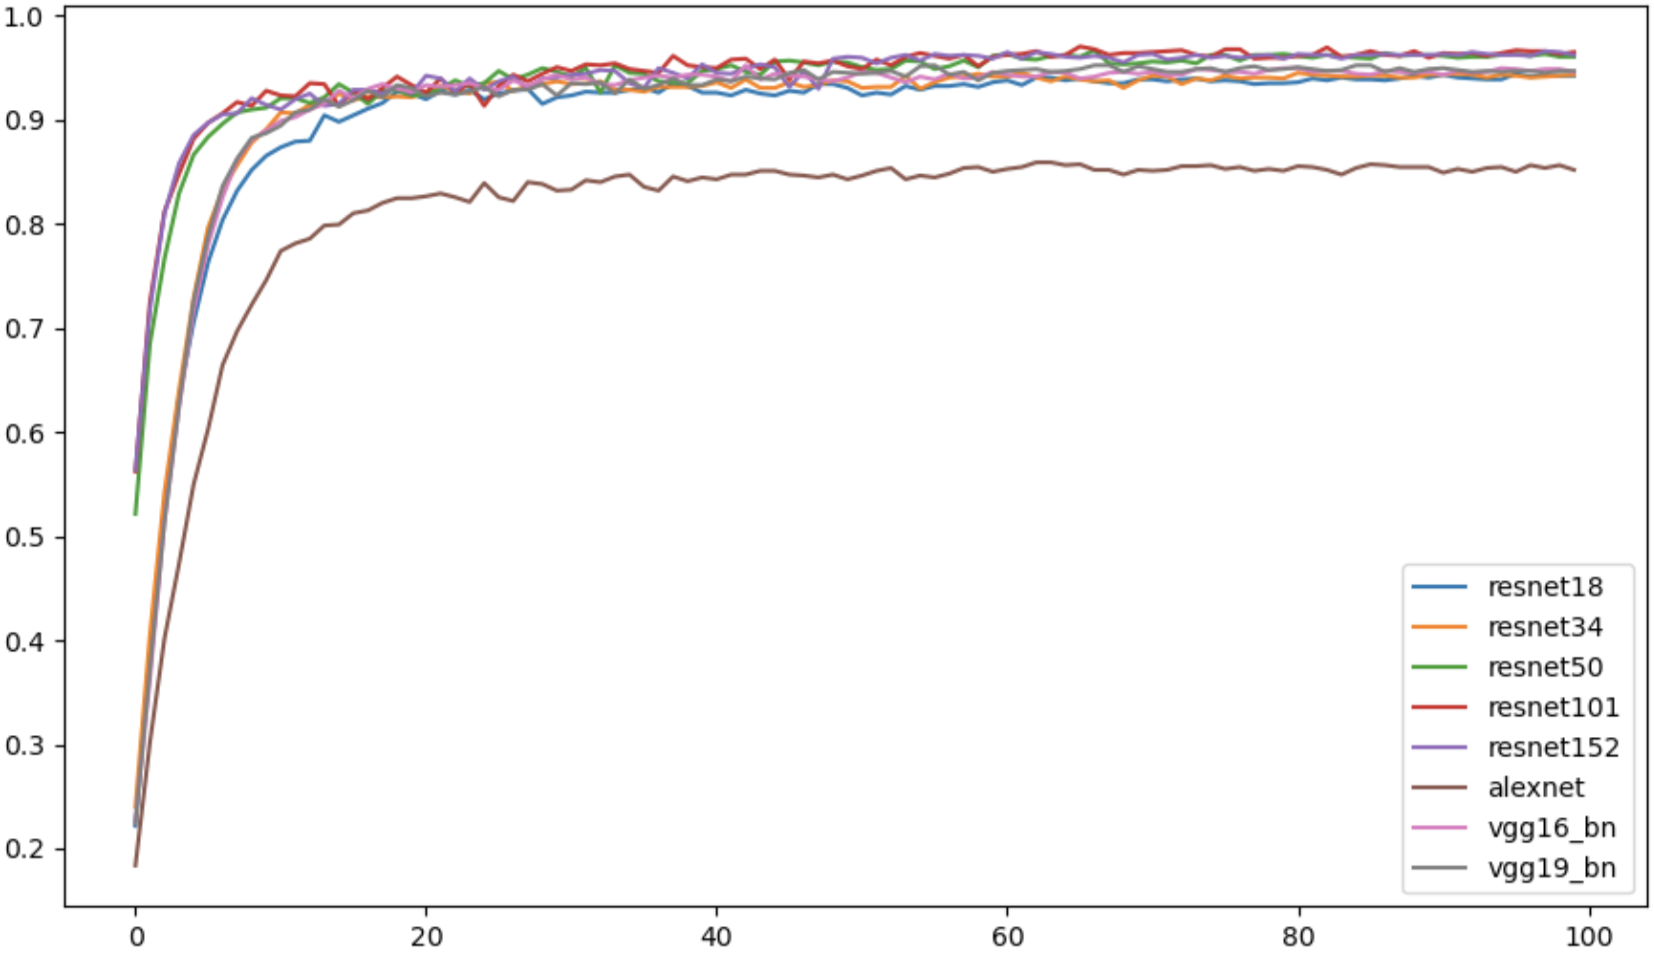
\includegraphics[width = 11 cm]{seedlings_100.png}
        \caption[Accuracy achieved by the models after being trained for 100 epochs]{Accuracy achieved by the models after being trained for 100 epochs. The x axis is the number of epochs, while the y axis is the accuracy achieved}
         \label{fig:seedlings_100_epoch_accuracy}
\end{figure}


\begin{table}[htbp]
\centering
\begin{tabular}{ p{2cm} p{4cm} p{3cm} p{3cm} p{2cm}  }
 Model& Top Accuracy (\%) & Epochs needed &Average Time (s)&Total Time (s)\\
 \hline
Resnet18&94.39&96&7&747\\
Resnet34&94.48&62&9&876\\
Resnet50&96.65&67&14&1439\\
Resnet101&97.01&66&21&2101\\
Resnet152&96.56&98&29&2851\\
Alexnet&85.88&63&7&705\\
VGG16&95.20&43&17&1743\\
VGG19&95.20&56&20&1952\\
 \hline
\end{tabular}
\caption{Performances of the models trained with the 'plant\_seedlings\_v2' dataset for 100 epochs}
\label{tab:performances_seeds}
\end{table}


Fig. \ref{fig:seedlings_100_epoch_accuracy} shows the response of all models during the training based on the epoch used for training. The response of the model shows that, within the first ten epochs, the accuracy increases quickly and tends to stabilise afterwards, increasing slowly over time. However, we can observe a compact graph, meaning all the models (besides Alexnet) achieved accuracies not too far off from each other.
As a matter of fact, the difference in accuracy between the highest performing model (Resnet101) and the lowest performing model (Resnet18) was only 3\%.  


Fig. \ref{fig:seedlings_100_acc}, on the other hand, depicts the accuracy graphed over training time. Alexnet took the least amount of time to finish the training cycle (747 seconds), however Resnet18 took only \textasciitilde40 seconds more and reached a far better accuracy(94\% compared to 85\%). Resnet152 took 47 Minutes and 30 Seconds (2851 seconds) to complete the test and is the model that required the most time. \\
\begin{figure}[h]
       \centering 
	    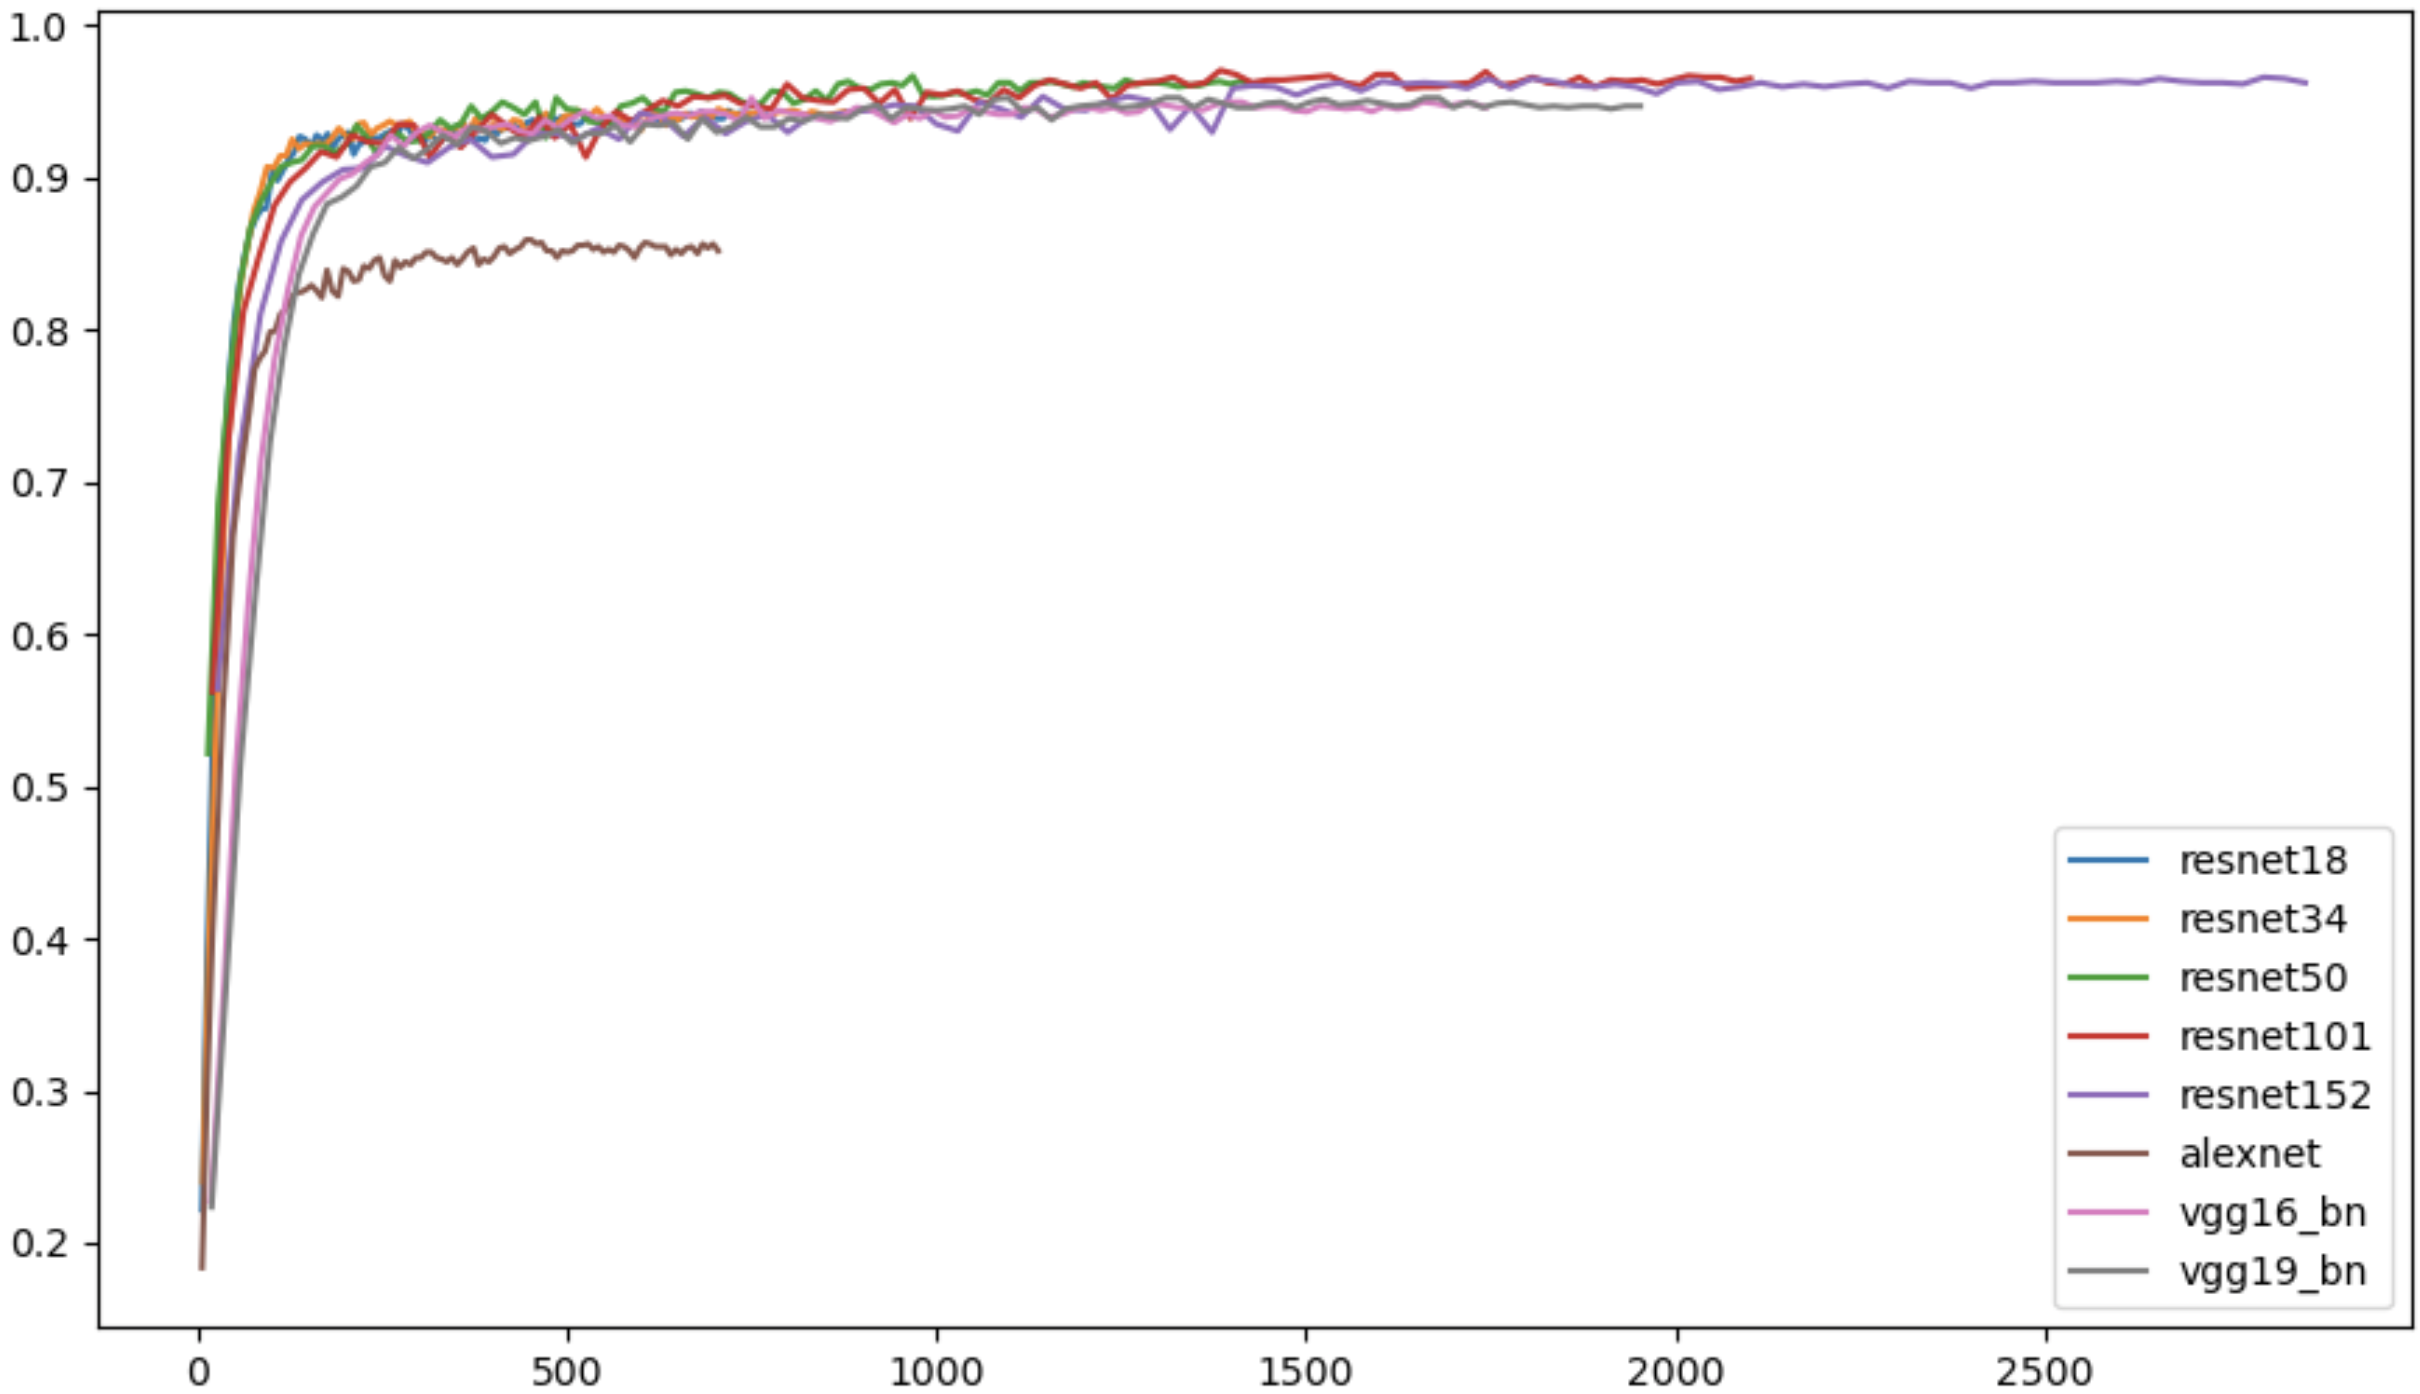
\includegraphics[width = 12 cm]{seedlings_100_acc.png}
        \caption[Accuracy achieved when training for 100 epochs in relation with training time]{Accuracy achieved when training for 100 epochs in relation with training time. The x axis is the training time in seconds, while the y axis is the accuracy achieved}
         \label{fig:seedlings_100_acc}
\end{figure}

\begin{figure}[h]
\begin{subfigure}{0.5\textwidth}
	    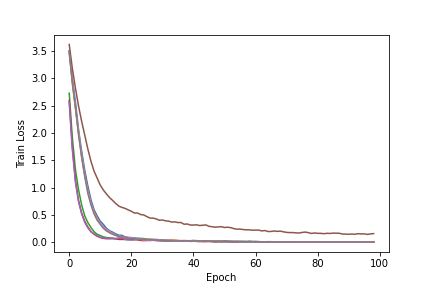
\includegraphics[width = \gws cm]{epoch_train_loss_seeds_100.png}
	    \caption{Training loss calculated over 100 epochs}
        \label{fig:train_loss_seeds_100}
     \end{subfigure} \hfill
     \begin{subfigure}{0.5\textwidth}
	    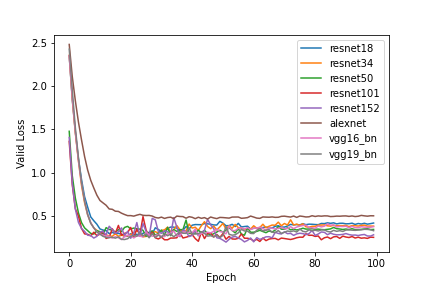
\includegraphics[width = \gws cm]{epoch_valid_loss_seeds_100.png}
	    \caption{Validation loss calculated over 100 epochs}
         \label{fig:valid_loss_seeds_100}
     \end{subfigure}
     
     \caption{Training loss and validation loss of all models calculated over 100 epochs}
        \label{fig:tran_valid_loss_seeds_100}
        
      
\end{figure}


In Fig. \ref{fig:tran_valid_loss_seeds_100}, we can analyse the loss calculated for the models during the training. As shown in Fig. \ref{fig:train_loss_seeds_100}, all the models (besides Alexnet) reached 0 loss within the first 30 epochs. This means that, theoretically, the models learned the dataset perfectly within the first 20 epochs. Usually, when the training loss is 0, we are expecting a case of over-fitting, which would be proven by a high validation loss. We can then study the validation loss of the models in Fig. \ref{fig:valid_loss_seeds_100}. From their response, we can observe that the validation loss does not increase drastically like we saw in the first experiment. On the contrary, we can see in table \ref{tab:difference_val_tra_loss} that the difference between validation loss and training loss is rarely more than 0.4. Furthermore, the curve seems to be quite stable, especially for shallower networks, and the validation loss tends to increase slowly. 
\begin{table}[h]
\centering
        \begin{tabular}{ c c  }
                 Model&Difference\\
                 \hline
                   Resnet18&0.42\\
                    Resnet34&0.38\\
                    Resnet50&0.35\\
                    Resnet101&0.25\\
                    Resnet152&0.28\\
                    Alexnet&0.34\\
                        VGG16&0.38\\
                    VGG19&0.33\\
                    \end{tabular}
                    \caption{Difference between validation loss and train loss after 100 epochs }                   
                     \label{tab:difference_val_tra_loss}
     \end{table} 

For example, we can analyse the trend for the model which reached the highest accuracy overall, namely Resnet101, shown in Fig. \ref{fig:epoch_valid_loss_resnet101}. As shown in table \ref{tab:difference_val_tra_loss}, the difference at the end of the training is 0.25. Moreover - as we suspected before - the training loss approaches zero within the first 30 epochs, while the validation loss remains stable for the entire training process, with some spikes at around the 30 epochs. Furthermore, the validation loss becomes higher than the training loss at around 10 epochs.\\
We can observe a similar behaviour in the response of Resnet152 (Fig. \ref{fig:epoch_valid_loss_resnet152}). The training loss approaches zero once more around the 30 epochs and becomes smaller than the validation loss at around 10. Although the validation loss tends to stabilise for this model, as well, the graph shows a less stable behaviour with more fluctuations between 20 and 50 epochs. \\
\begin{figure}[h]
\begin{subfigure}{0.5\textwidth}
     \centering
	    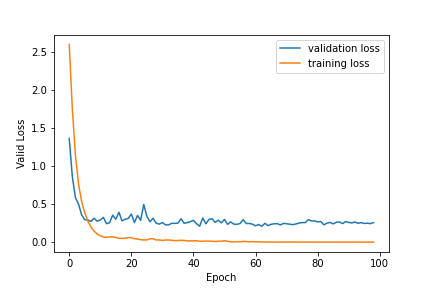
\includegraphics[width = \gws cm]{epoch_valid_loss_resnet101.png}
\caption{Resnet101}\label{fig:epoch_valid_loss_resnet101}
     \end{subfigure}
\begin{subfigure}{0.5\textwidth}
     \centering
	    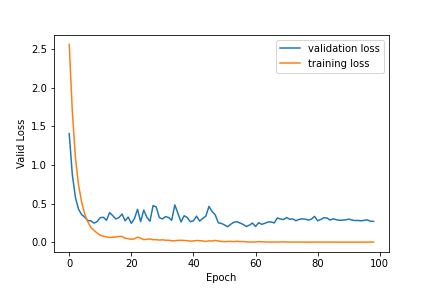
\includegraphics[width = \gws cm]{epoch_valid_loss_resnet152.png}
\caption{Resnet152}\label{fig:epoch_valid_loss_resnet152}
     \end{subfigure}  
     \caption{Training loss and validation loss of Resnet101 and Resnet152 over 100 epochs}
        \label{fig:tran_valid_loss_seeds_res_100}
\end{figure}

In addition to the training time, we can also use the benchmark tool we developed to measure and analyse the inference time of each model.\\
As we are mostly focused on sugar beet recognition, it is safe to assume use cases where field robots would scan the field to recognize the vegetation, similarly to the one proposed by \textit{Lottes et al.} in \cite{7487720}. In such setting, the time taken to classify the image, ultimately, results in a soft deadline, as the time taken to scan the field is greatly influenced by it, therefore being able to estimate the needed inference time could help optimise this part of the application. \\
In order to test for inference time, we are going to use a dataset composed of \textasciitilde120 pictures taken from the original dataset. These pictures were taken before starting the process, therefore they have not been used for training.The results are shown in Fig. \ref{fig:inf_time_epoch_seeds}.\\ Fig. \ref{fig:inf_acc_models_seeds} shows the inference time based on the accuracy, while figure \ref{fig:inf_epoch_models_seeds} shows the inference time based on the epoch used to train. \\
From Fig. \ref{fig:inf_acc_models_seeds} we can start to observe some rather interesting properties. For each model, as they achieve accuracy less than 88\%, the inference time is rarely measured to be more than 60 ms, with only 2 exceptions (\textasciitilde100ms and \textasciitilde390ms). Furthermore, the only model that achieved an accuracy smaller than \textasciitilde82\% is Alexnet\footnote{The whole results can be seen in Fig. \ref{fig:accuracy_inferencetime_seedlings}}.
\begin{figure}[h]
     \begin{subfigure}{0.5\textwidth}
	    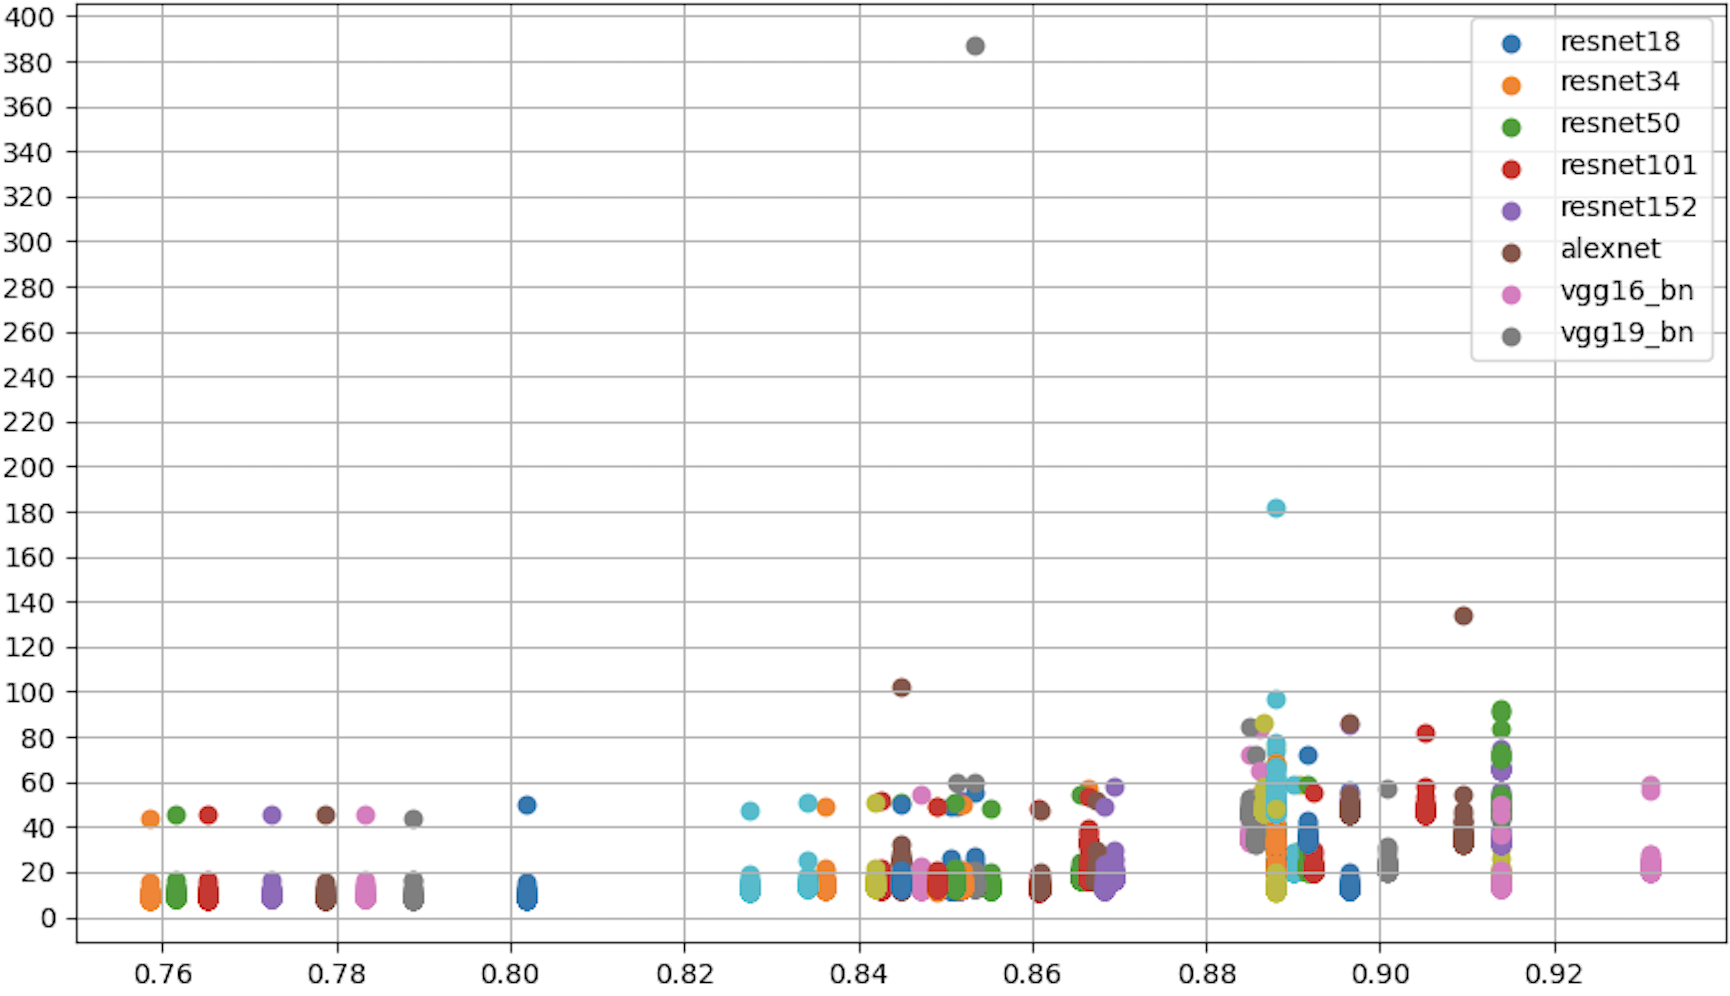
\includegraphics[width = \gws cm]{inf_acc_models_seeds.png}
	    \caption{Based on accuracy}
         \label{fig:inf_acc_models_seeds}
     \end{subfigure}
     \hfill
     \begin{subfigure}{0.5\textwidth}
	    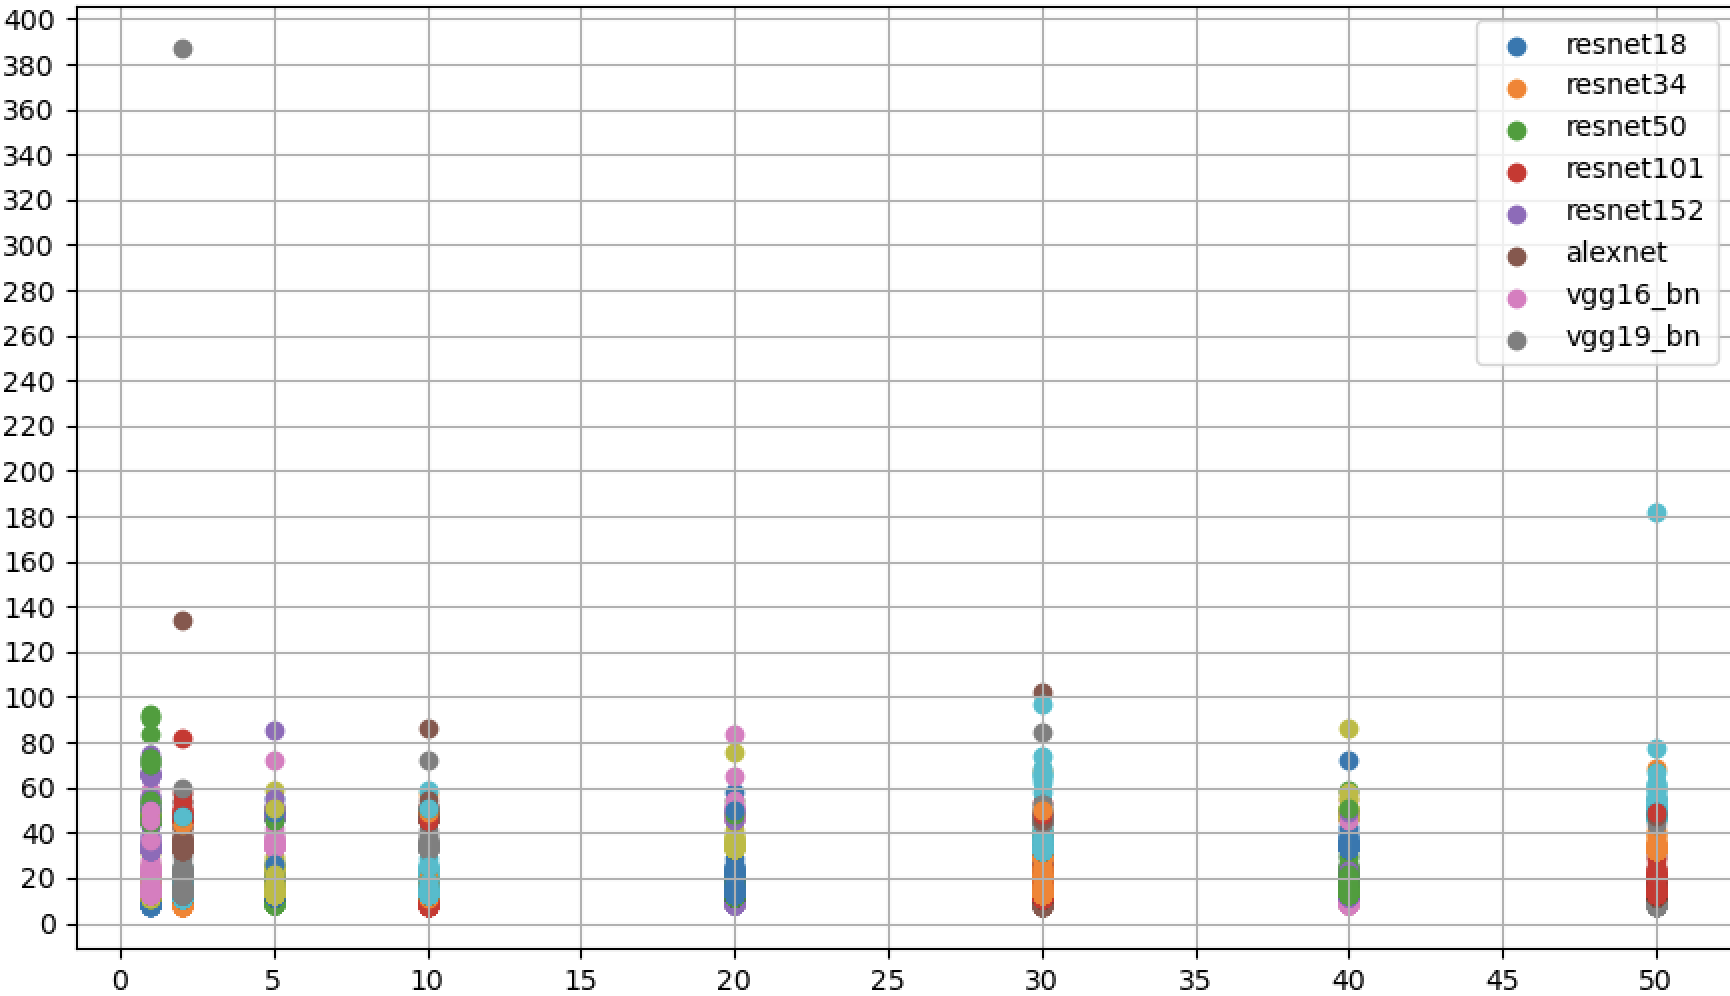
\includegraphics[width = \gws cm]{inf_epoch_models_seeds.png}
	    \caption{Based on the number of epochs}
        \label{fig:inf_epoch_models_seeds}
     \end{subfigure}\\
     \caption[Inference time measured for each model]{Inference time measured for each model using the dataset discussed previously. The inference time is in milliseconds, while the accuracy for Fig. \ref{fig:inf_time_accuracy}is the percentage of correct predictions.}
        \label{fig:inf_time_epoch_seeds}
\end{figure}


For accuracies over 88\%, although the behaviour of the models seems to be less compact, the inference time rarely measures more than 100 milliseconds, with only two outliers(\textasciitilde135ms and \textasciitilde180s).\\
From Fig. \ref{fig:inf_epoch_models_seeds} we can see that, with the exception of the outliers we identified before, the number of epochs that measured the highest value for inference is 30. As a matter of fact, when trained for different numbers of epochs, the models never require more than 100 milliseconds to process the images. 
\begin{figure}[h]
     \begin{subfigure}{0.5\textwidth}
	    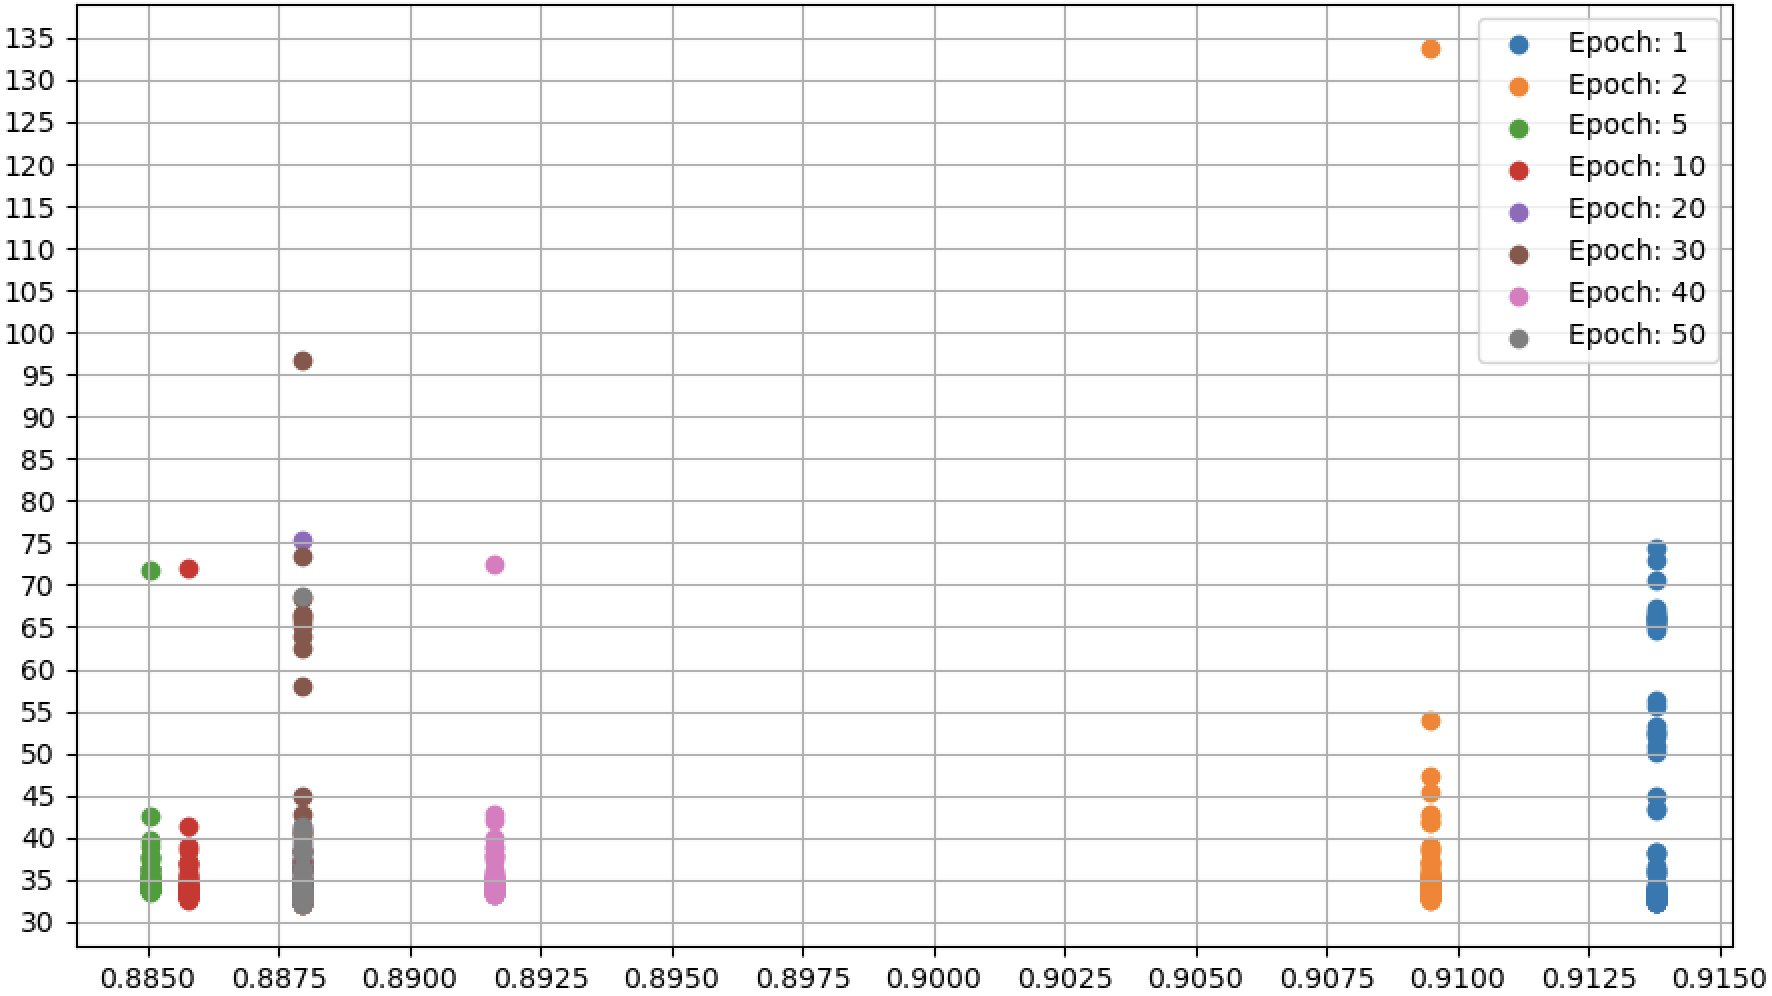
\includegraphics[width = \gws cm]{inf_resnet101_seeds.png}
	    \caption{Resnet101}
         \label{fig:inf_resnet101_seeds}
     \end{subfigure}
     \hfill
     \begin{subfigure}{0.5\textwidth}
	    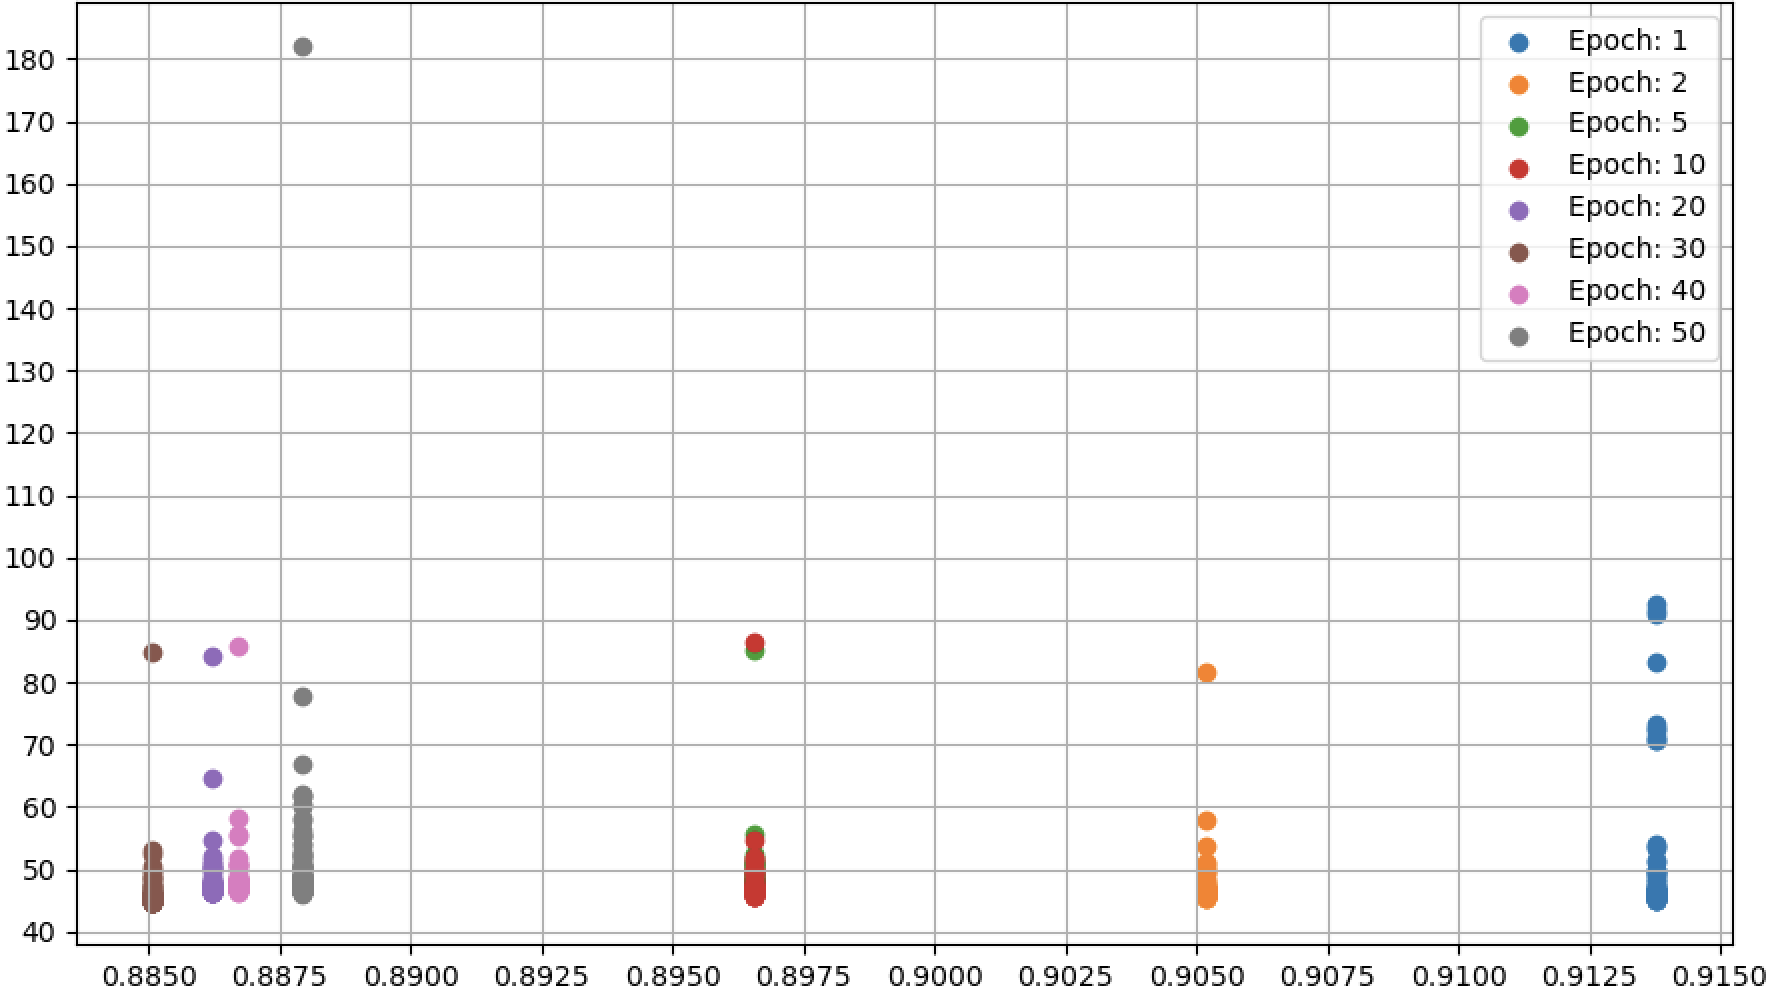
\includegraphics[width = \gws cm]{inf_acc_152_seeds.png}
	    \caption{Resnet152}
        \label{fig:inf_acc_152_seeds}
     \end{subfigure}\\
     \caption[Inference time measured for Resnet101 and Resnet152]{Inference time measured for Resnet101 and Resnet152. The inference time is in milliseconds, while the accuracy is the percentage of correct predictions.}
        \label{fig:inf_time_epoch_seeds2}
\end{figure}



A closer investigation of the individual performance of each model shows further interesting aspects. For the purpose of this experiment, we are going to analyse only Resnet101 and Resnet152, whose behaviour is shown in Fig. \ref{fig:inf_resnet101_seeds} and Fig. \ref{fig:inf_acc_152_seeds} respectively. For both models, we can see that the highest accuracy is achieved when trained for only one (\textasciitilde91\% for both) and two epochs (slightly lower of 91\% for Resnet18 and \textasciitilde90\% for Resnet152). For the other epoch, the accuracy achieved was consistently lower than 90\%. \\
In the case of Resnet101, the fastest training time has been achieved when trained for ten and five epochs, with an inference time of over 45 milliseconds on only two occasions. Although the fastest, the model trained with these epochs also achieved the lowest accuracy. The slowest inference time has been achieved when the model has been trained for two epochs, with an inference as high as 135 milliseconds. However, the model achieved the worst performance when trained for 30 epochs. As a matter of fact, even though it measured the lowest inference time when trained for two epochs, this occurred in only one case, while, when trained for 30 epochs, for a considerable amount of pictures, the inference time was in a range between 57 and 95 milliseconds. \\
Resnet152, on the other hand, showed more consistent results, with an inference time being in the range of 40 to 90 milliseconds for all epochs with the exception of one case where it reached 180 milliseconds. The fastest inference time for this model is measured when the model has been trained for 20 epochs.\\
From this investigation we can conclude that the performances of these two models are quite comparable, when it comes to inference. Both in terms of inference time and accuracy achieved, the two models show similar results, albeit for different levels of training. \\
For example, in the case of Resnet152, with a training time of 580 seconds (20 epochs), we obtain a model that can make predictions in a range between 45 and 85 milliseconds with an accuracy of \textasciitilde89\%. In the case of Resnet101, we can obtain similar results (prediction time between 70 and 30 milliseconds with an accuracy of \textasciitilde89\%) with a training time of 210 seconds (10 epochs). \\

\begin{figure}[h]
       \centering 
	    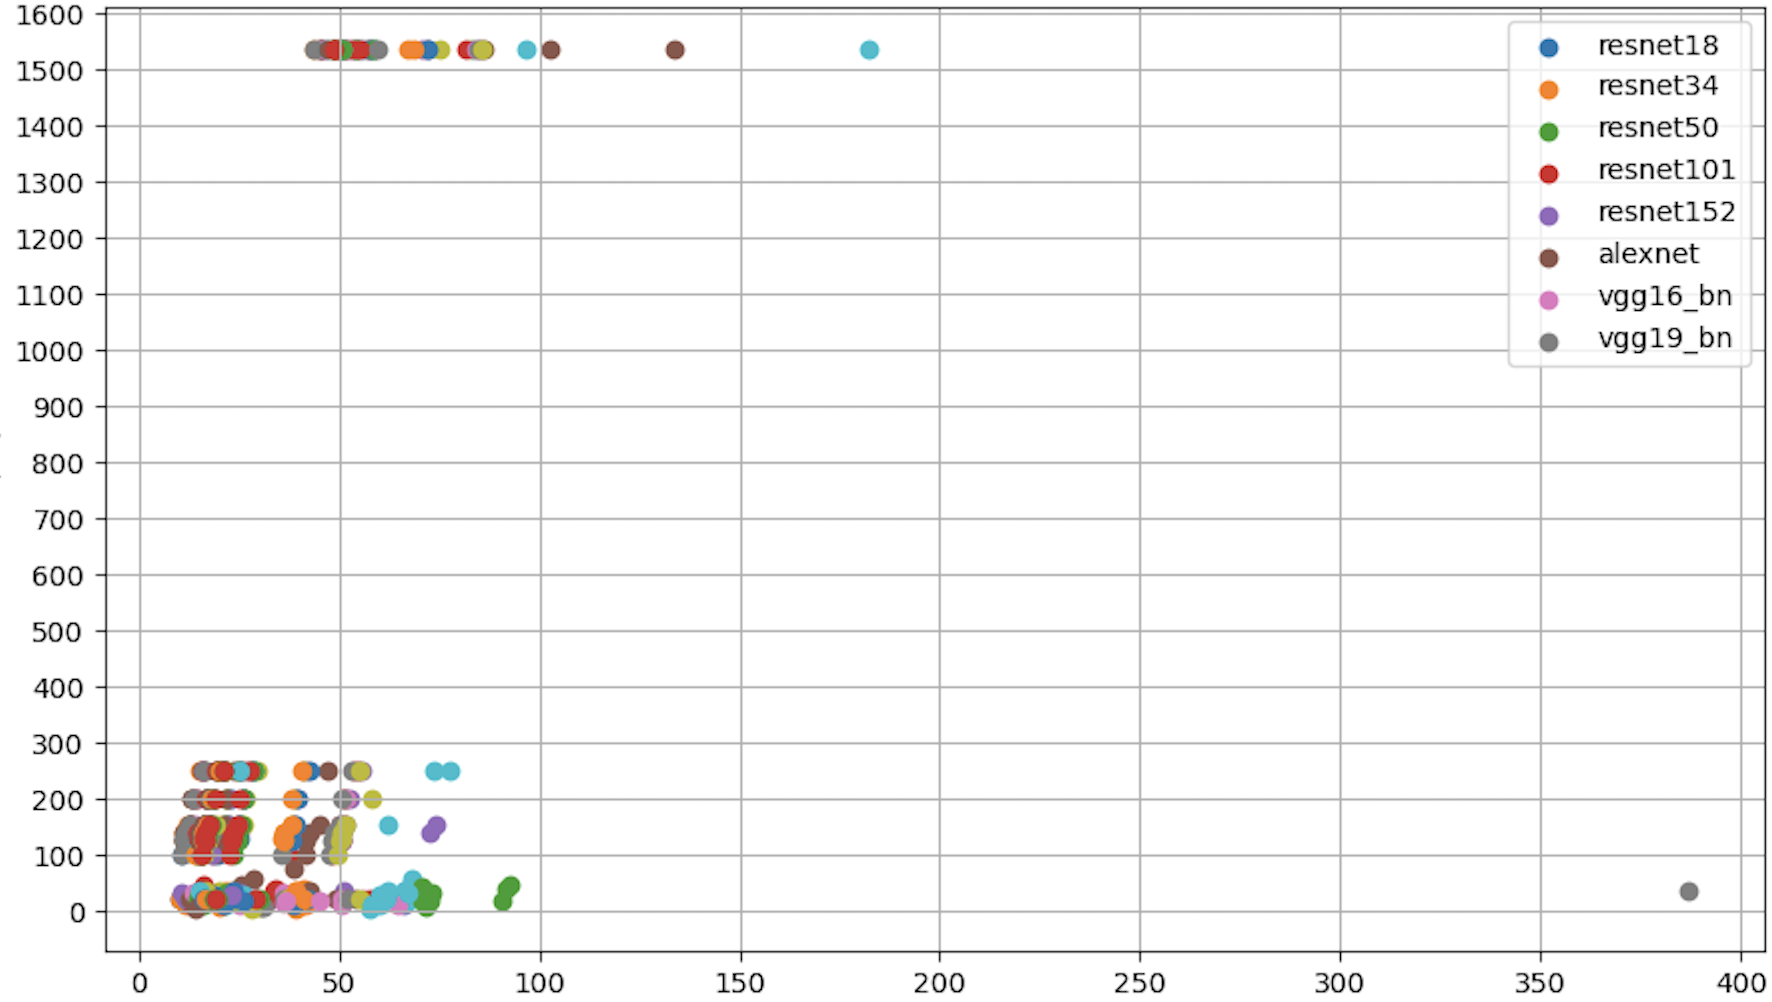
\includegraphics[width = 14 cm]{inf_size_seeds.png}
        \caption[Size of the images over inference time for the seedlings dataset]{This graph shows the size in kb (y axis) of the ten slowest images over the time taken to be processed (x axis)}
         \label{fig:inf_size_seeds}
\end{figure}

We can also run the tool to discover which pictures took the most amount of time to be processed. Fig. \ref{fig:inf_size_seeds} shows the ten slowest images for each model graphed based on their sizes. \\
The graph shows a rather compact and stable behaviour, with the slowest time measured for images having a size bigger than 1500 kb. \\
For pictures of more than 100 kb and less than 300 kb, the inference time is between 0 and 100 ms, with each model performing rather similarly. \\
For this experiment, both for training and for testing inference, we used a dataset with images having rather similar size and resolution, therefore this analysis is not as valuable as expected.\\
However, we can run the tool to make modifications on the images of the dataset. As a matter of fact, the tool also allows one to make a copy of the pictures in the dataset and transform them into grey-scale. Therefore, we can double the amount of pictures in the dataset by including grey-scale copies of those. \\
The results of the first run are shown in table \ref{tab:performances_seeds_gray}. When compared to 
table \ref{tab:performances_seeds}, we can observe that all the models have reached better accuracy besides Alexnet. As a matter of fact, Alexnet peaked at \textasciitilde80\%, while all the other models peaked at accuracies over 95\%. The best accuracy has been achieved by Resnet101 (\textasciitilde99\%) in 80 epochs. Furthermore, this time around, in comparison to the previous run, all the models took more time to train, with a difference in average time for epoch being from one second (Alexnet) to 23 seconds (Resnet152). This is the result of introducing more pictures in the dataset, which makes the training process more time-consuming. \\
\begin{table}[htbp]
\centering
\begin{tabular}{ p{2cm} p{4cm} p{3cm} p{3cm} p{2cm}  }
 Model& Top Accuracy (\%) & Epochs needed &Average Time (s)&Total Time (s)\\
 \hline
Resnet18&95.98&82&9.16&916\\
Resnet34&96.72&90&12.67&1267\\
Resnet50&98.15&82&23.66&2366\\
Resnet101&99.12&80&37.05&3705\\
Resnet152&98.84&85&52.01&5201\\
Alexnet&79.81&89&8.12&812\\
VGG16&97.27&93&29.87&2987\\
VGG19&96.77&64&33.74&3374\\
 \hline
\end{tabular}
\caption{Performance of the models trained for 100 epochs on the 'plant\_seedlings\_v2' dataset including the grey-scale variant of the pictures}
\label{tab:performances_seeds_gray}
\end{table}


The analysis of the training loss and validation loss trends also offers quite different results. An overview can be seen in table \ref{tab:difference_val_tra_loss_2}. The difference in loss between the validation and the training set decreased quite substantially. For example, Resnet101 and Resnet152, which were also the ones with the lowest difference in the previous run (see table \ref{tab:difference_val_tra_loss_2}), measured a difference of only 0.07 and 0.08 respectively. \\
Fig. \ref{fig:tran_valid_loss_seeds_res_100_2} shows the trend for the two models. We can observe that the training loss approaches zero after around 30 epochs, while the validation loss tends to decrease further and stabilises after around 80. It is also worth pointing out that, in the case of Resnet101, the validation loss starts to increase after around 10 epochs and, since the training loss is already approaching zero, it would satisfy the criteria for an early stopping of the training. However, right after the 20 epochs mark, the validation loss decreases once again, up until it becomes only slightly larger than the training and then stabilises afterwards. 

\begin{table}[h]
\centering
        \begin{tabular}{ c c  }
                 Model&Difference\\
                 \hline
                   Resnet18&0.20\\
Resnet34&0.18\\
Resnet50&0.12\\
Resnet101&0.07\\
Resnet152&0.08\\
Alexnet&0.20\\
VGG16&0.12\\
VGG19&0.14\\
                    \end{tabular}
                    \caption{Difference between validation loss and train loss after 100 epochs using the gray-scale variants of the pictures}                   
                     \label{tab:difference_val_tra_loss_2}
     \end{table} 
     
     
\begin{figure}[h]
\begin{subfigure}{0.5\textwidth}
     \centering
	    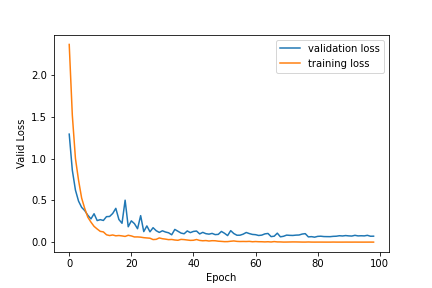
\includegraphics[width = \gws cm]{epoch_valid_loss_resnet101_2.png}
\caption{Resnet101}\label{fig:epoch_valid_loss_resnet101_2}
     \end{subfigure}
\begin{subfigure}{0.5\textwidth}
     \centering
	    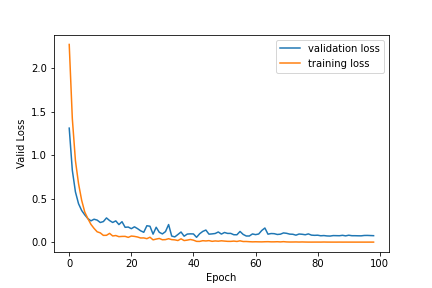
\includegraphics[width = \gws cm]{epoch_valid_loss_resnet152_2.png}
\caption{Resnet152}\label{fig:epoch_valid_loss_resnet152_2}
     \end{subfigure}  
     \caption{Training loss and validation loss of Resnet101 and Resnet152 over 100 epochs on the  'plant\_seedlings\_v2' dataset and the grey-scale variant of the pictures}
        \label{fig:tran_valid_loss_seeds_res_100_2}
\end{figure}
From the information acquired so far, we would expect the models to perform better during the inference time test. Fig. \ref{fig:inf_seeds_with_grey} shows the results of the tests. In Fig. \ref{fig:inf_seeds_grey_no_grey}, the performance of the models has been tested using the same inference dataset we used for the results in Fig. \ref{fig:inf_acc_models_seeds}. Comparing the two graphs, we can observe that the accuracy dropped significantly. As a matter of fact, without the grey images for training, the lowest accuracy achieved was around \textasciitilde75\%, while in this run we calculated accuracies at around \textasciitilde69\%. Furthermore, the highest accuracy calculated in this run is around \textasciitilde88\%,
while in the run before the highest achieved was \textasciitilde92\%. The inference time did not improve as well, as the models showed a comparable or oven worst response time for the images at each epoch. Interestingly, when we observe the overall trend of the models, we can see that as the accuracy increases, it appears that they require more time to process the images and make their predictions.\footnote{The whole results can be seen in Fig. \ref{fig:accuracy_inferencetime_seedlings_grey_train}}\\

\begin{figure}[h]
     \begin{subfigure}{0.5\textwidth}
	    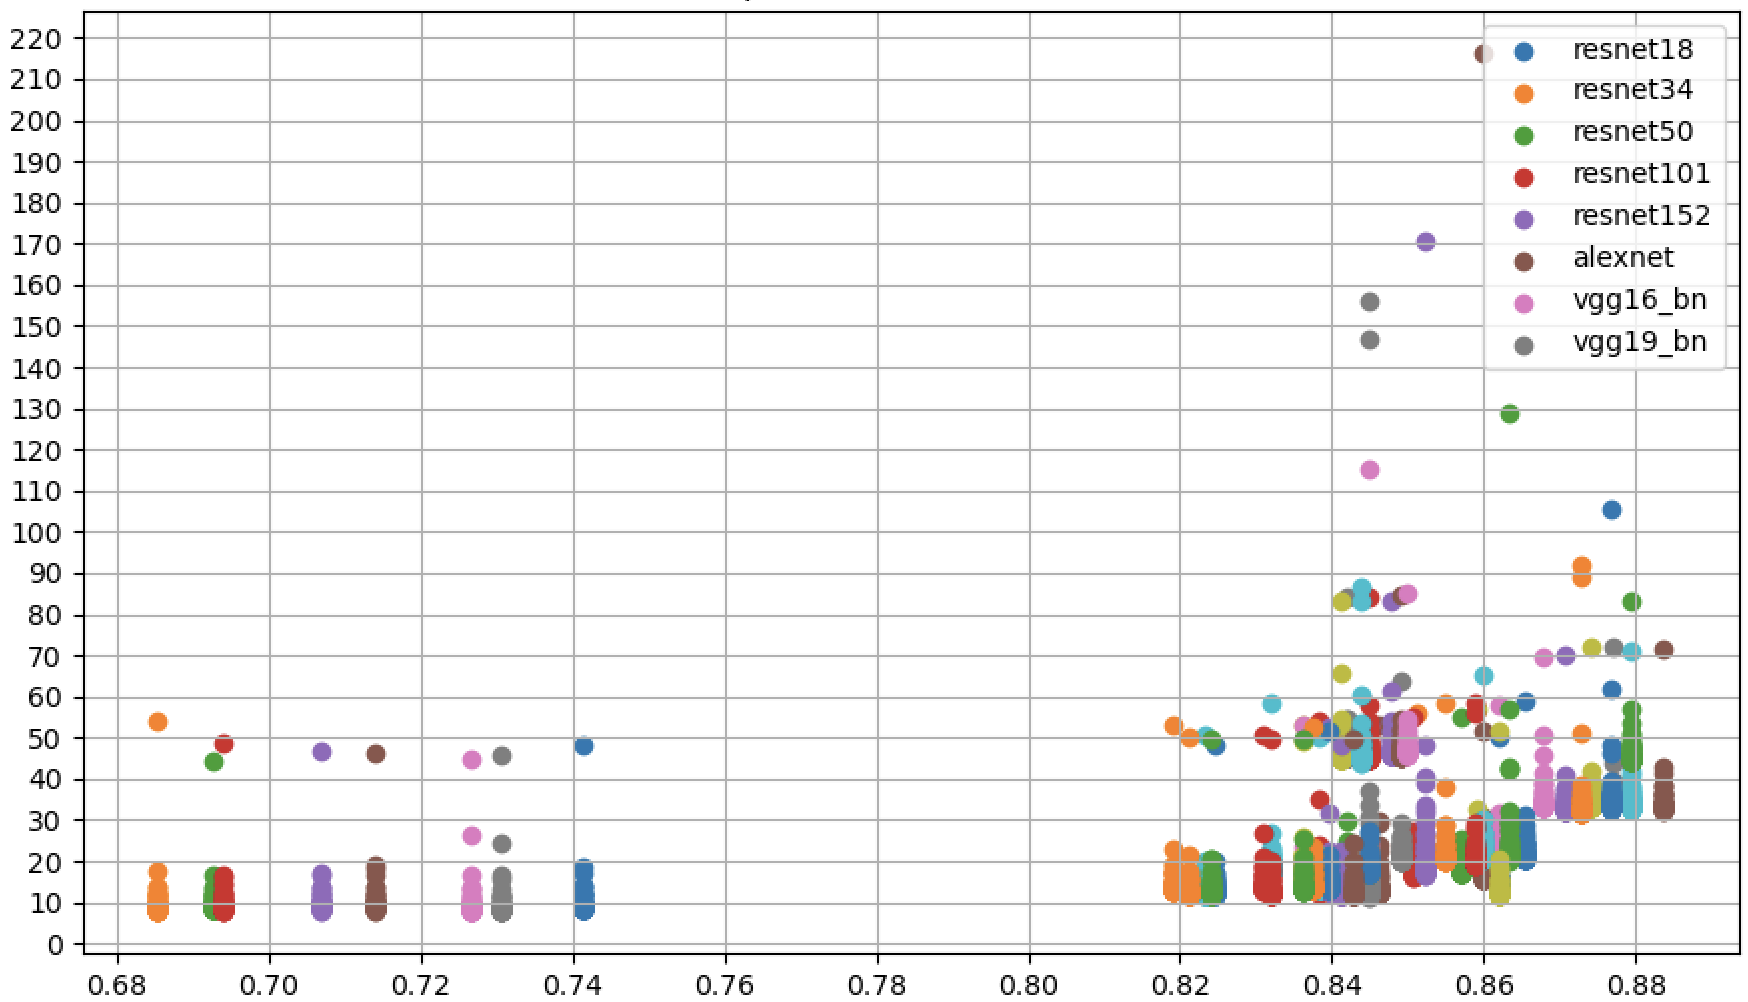
\includegraphics[width = \gws cm]{inf_seeds_grey_no_grey.png}
	    \caption{}
         \label{fig:inf_seeds_grey_no_grey}
     \end{subfigure}
     \hfill
     \begin{subfigure}{0.5\textwidth}
	    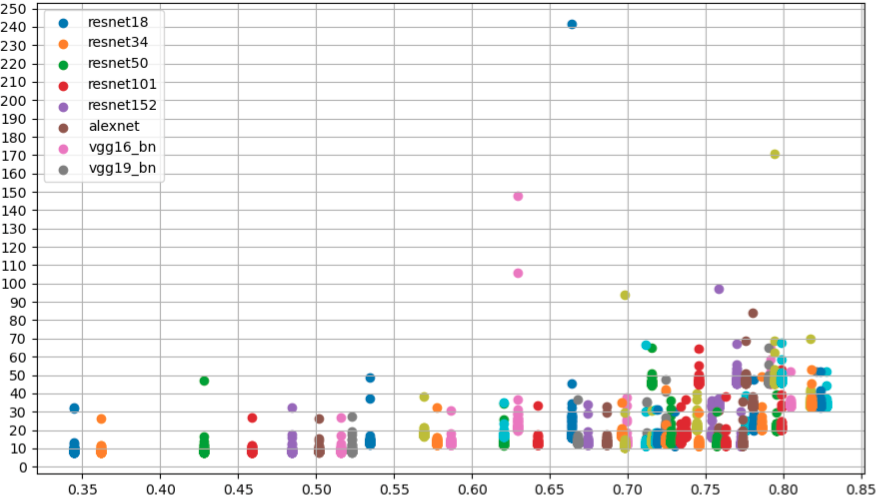
\includegraphics[width = \gws cm]{inf_acc_seeds_grey_img.png}
	    \caption{}
        \label{fig:inf_acc_seeds_grey_img}
     \end{subfigure}\\
     \caption[Inference time of each model trained with grey images as well]{Inference time of each model trained with grey images as well. In Fig. \ref{fig:inf_seeds_grey_no_grey}, the inference is calculated using the same dataset used in Fig. \ref{fig:inf_acc_models_seeds}, while in Fig.  \ref{fig:inf_acc_seeds_grey_img} the dataset is composed with the same pictures, but in grey scale. }
        \label{fig:inf_seeds_with_grey}
\end{figure}


From Fig. \ref{fig:inf_acc_seeds_grey_img},on the other hand, we can see the inference time of the models using the same image we used before, but in grey-scale. In this run, the accuracy dropped to a lowest point of \textasciitilde35\%, a considerable downgrade from the \textasciitilde75\% of the original run. The highest accuracy, on the other hand, dropped to \textasciitilde85\%, i.e. similar to the \textasciitilde88\% of before. In this run, the overall inference time failed to improve, as well, but rather tended to increase as the accuracy increases.\footnote{The whole results can be seen in Fig. \ref{fig:accuracy_inferencetime_seeds_grey}} \\

From these analyses we can conclude that, for this dataset and for these models, including grey-scale versions of the images increases the performances in training, but negatively effects the inference performances of the models. 
